

\chapter{A simple model of the sodium channel \label{simple_Na}}

In the previous two chapters, we studied a prototypical model of an ion
channel. The model consisted of a differential equation involving a gating
mechanism that could be either open or closed. A Markov model governed the
gating and we derived a system giving the probability density functions of
the states involved in the Markov model. We used the probability density
approach to compute optimal theoretical drugs and noted that a mutation
leading to an increase in the closed to open reaction rate could be completely
repaired by an optimal closed state drug.

Next, we extended the prototypical model to also include an inactivated state.
The inactivated state can also be affected by mutations and we studied the
particular case in which the rates from inactivated to open and from 
inactivated to closed were increased by a factor $\mu$ referred to as the 
mutation severity index. In this case, we observed that an optimal drug was 
represented by a blocker associated with the inactivated state. We were again
able to completely repair the effect of the mutation using the theoretical
 drug.

In this chapter, we shall move closer to realistic Markov models of sodium
channels. These models tend to be somewhat more intricate than the
prototypical model we have studied so far. Providing Markov models of the
sodium channels has been a very active field of research for decades and a
series of models are available. We have chosen to study models that seem to
capture the basic structure applied in many models but are manageable from a
mathematical point of view. We choose this approach for clarity of
presentation and not for its ability to represent specific data. It is,
hopefully, quite clear that the method we use to analyze the models is
applicable to many other models.

Mutations of the sodium channel can lead to impaired inactivation. This may
lead to leakage of the sodium current, which can again trigger arrhythmias.
Here we will consider a model of the $\Delta$KPQ mutation of the SCN5A gene.
This mutation may lead to an arrhythmogenic disorder referred to as the long-QT
syndrome, which can lead to sudden cardiac death in the worst case. There are
several models representing the effect of the $\Delta$KPQ mutation. 
One that is well known is
provided by Clancy and Rudy \cite{Clancy1999}. Their approach to model the
impaired inactivation is to introduce a burst mode in the model where no
inactivation state is available. We will consider two ways of modeling the
effect of the mutation.

 In the first approach, we will use the method
utilized above. We will simply increase the reaction rate from the inactivated
to the closed state and from the inactivated to the open state by a factor
$\mu\ge1$, referred to as the mutation severity index. This change will clearly
reduce the probability of being in the inactivated state. 
It is therefore a model of impaired inactivation.

The second approach is
to introduce a burst mode in the model. When the channel is in the burst mode,
there is no inactivated state. This model will be
parameterized such that it is highly unlikely that the channel will enter the
burst mode for the wild type case, but the probability of entering the burst
mode is considerably higher in the mutant case.

\section{Markov model of a wild type sodium channel}

Markov models have turned out to be a powerful tool in representing the physics
of the sodium channel and a series of alternatives have been proposed by
various authors. Since this is still a very active field of research, it is hard
to claim one particular model as the definitive model. We
shall therefore focus on a kind of model that has a structure that seems to
be more or less agreed upon but, as usual, we attack this problem with
simplicity in mind. This also holds true for the way we introduce the effect
of a mutation.

We start by considering a simple model of the sodium channel, illustrated in
Figure \ref{wtreac}. The actual functions used in our computations will be
given below. However, we should note that the functions will always be chosen
such that they satisfy the principle of detailed balance, which, for the model
given in Figure \ref{wtreac}, means that the following relation holds:%
\begin{equation}
k_{io}k_{oc}k_{ci}=k_{oi}k_{ic}k_{co}. \label{db2}%
\end{equation}
The model of the closed states deserves a comment or two. Let us assume that a
sodium channel consists of three subunits and these subunits may exist in two
states: closed or permissible. The whole channel is in the state $C_{0}$ if
all three units are in the permissible state. Over a brief period given
by $\Delta t$, the channel can change from the state $C_{0}$ to the open
state and the probability of this event is $\Delta t k_{co}$ or it can
change to the inactivated state with probability $\Delta t k_{ci}$. However, the
channel can also go from the permissible state $C_{0}$ to the state $C_{1}$ and 
the probability of doing this is $3\Delta t \beta$. The reason for the factor 
of three here is that it is sufficient that one of the three subunits closes. By
assuming that the subunits act independently, we find that the probability is
$3\Delta t \beta$. The same reasoning gives us the rest of the
transitions between the different closed states.

\begin{figure}[ptb]
\begin{center}
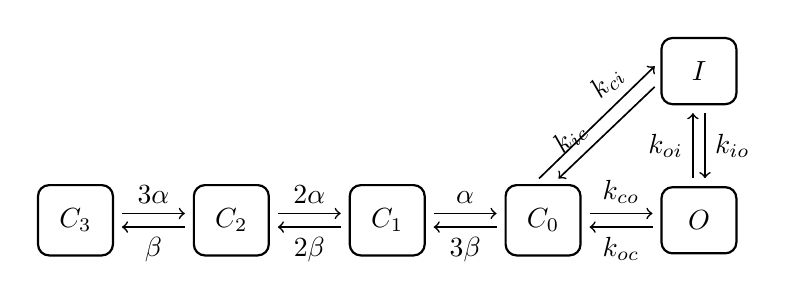
\begin{tikzpicture}[
   font=\sffamily,
   every matrix/.style={ampersand replacement=\&,column sep=1cm,row sep=1cm},
   state/.style={draw,thick,rounded corners,inner sep=.3cm},
   to/.style={->,semithick,shorten >=0.1cm,shorten <=0.1cm},
   Q/.style={->,semithick,sloped,pos=0.700000,shorten >=0.1cm,shorten <=0.1cm}, 
   every node/.style={auto}]
\matrix{
\&\&\&\&\node[state] (I) {\parbox{10pt}{\centerline{$I$}}};\\
\node[state] (C_{3}) {\parbox{10pt}{\centerline{$C_{3}$}}};\&\node[state] (C_{2}) {\parbox{10pt}{\centerline{$C_{2}$}}};\&\node[state] (C_{1}) {\parbox{10pt}{\centerline{$C_{1}$}}};\&\node[state] (C_{0}) {\parbox{10pt}{\centerline{$C_{0}$}}};\&\node[state] (O) {\parbox{10pt}{\centerline{$O$}}};\\
};
\draw[to]  (O.100) to node {$k_{oi}$} (I.260);
\draw[to]  (O.190) to node {$k_{oc}$} (C_{0}.350);
\draw[to]  (I.280) to node {$k_{io}$} (O.80);
\draw[Q]  (I.195) to node {$k_{ic}$} (C_{0}.75);
\draw[to]  (C_{0}.10) to node {$k_{co}$} (O.170);
\draw[Q]  (C_{0}.105) to node {$k_{ci}$} (I.165);
\draw[to]  (C_{0}.190) to node {$3\beta$} (C_{1}.350);
\draw[to]  (C_{1}.10) to node {$\alpha$} (C_{0}.170);
\draw[to]  (C_{1}.190) to node {$2\beta$} (C_{2}.350);
\draw[to]  (C_{2}.10) to node {$2\alpha$} (C_{1}.170);
\draw[to]  (C_{2}.190) to node {$\beta$} (C_{3}.350);
\draw[to]  (C_{3}.10) to node {$3\alpha$} (C_{2}.170);
\end{tikzpicture}
\end{center}
\caption{Markov model of a wild type sodium channel consisting of an open
state $(O)$, an inactivated state $(I)$, and four closed states $(C_{0}%
,C_{1},C_{2},C_{3})$.}%
\label{wtreac}%
\end{figure}


\subsection{The equilibrium solution}

The equilibrium probabilities of the model given in Figure \ref{wtreac} are
characterized by the equations%
\[%
\begin{array}
[c]{ccc}%
k_{ci}c_{0}=k_{ic}i, & k_{oi}o=k_{io}i, & k_{co}c_{0}=k_{oc}o,\\
3\beta c_{0}=\alpha c_{1}, & 2\alpha c_{2}=2\beta c_{1}, & 3\alpha c_{3}=\beta
c_{2},
\end{array}
\]
where $c_{0}$ denotes the equilibrium probability of being in the state
$C_{0}$. Similarly, the other variables are defined as the equilibrium
probability of being in the states $C_{1},C_{2},C_{3},I$, and $O$. We express all
probabilities in terms of the open probability:%
\begin{align*}
i  &  =\frac{k_{oi}}{k_{io}}o,\text{ }c_{0}=\frac{k_{oc}}{k_{co}}o,\text{ }\\
c_{1}  &  =\frac{3\beta}{\alpha}\frac{k_{oc}}{k_{co}}o,\text{ }c_{2}%
=\frac{3\beta^{2}}{\alpha^{2}}\frac{k_{oc}}{k_{co}}o,\text{ }c_{3}=\frac
{\beta^{3}}{\alpha^{3}}\frac{k_{oc}}{k_{co}}o.
\end{align*}
Since $o+i+c_{0}+c_{1}+c_{2}+c_{3}=1,$ we find the following equilibrium probabilities:%

\begin{align}
o  &  =\frac{1}{q_{w}},\text{ }i=\frac{k_{oi}/k_{io}}{q_{w}},\text{ }%
c_{0}=\frac{k_{oc}/k_{co}}{q_{w}}, \label{prob_wt}\\
c_{1}  &  =\frac{3\beta}{\alpha}\frac{k_{oc}/k_{co}}{q_{w}},\text{ }%
c_{2}=\frac{3\beta^{2}}{\alpha^{2}}\frac{k_{oc}/k_{co}}{q_{w}},\text{ }%
c_{3}=\frac{\beta^{3}}{\alpha^{3}}\frac{k_{oc}/k_{co}}{q_{w}},\nonumber
\end{align}
where%
\[
q_{w}=1+\frac{k_{oi}}{k_{io}}+\frac{k_{oc}}{k_{co}}\left(  1+\beta
/\alpha\right)  ^{3}.
\]
Here the subscript $w$ is used to indicate that $q_{w}$ represents the 
wild type case.

\section{Modeling the effect of a mutation impairing the inactivated state}

The mutation impairs the inactivated state of the channel. In Section
\ref{mutaffectinactiv} we modeled this by increasing the probability of moving
from the inactivated state to the open state or to the closed state. This was
done by increasing the rates $k_{io}$ and $k_{ic}.$ We use the same approach
here and define%
\begin{align}
\bar{k}_{ic}  &  =\mu k_{ic},\label{kic1}\\
\bar{k}_{io}  &  =\mu k_{io}, \label{kio2}%
\end{align}
where, as usual, $\mu$ is the mutation severity index. From (\ref{db2}), we
have
\[
k_{io}k_{oc}k_{ci}=k_{ic}k_{co}k_{oi}%
\]
and therefore%
\[
\left(  \mu k_{io}\right)  k_{oc}k_{ci}=\left(  \mu k_{ic}\right)
k_{co}k_{oi};%
\]
so%
\[
\bar{k}_{io}k_{oc}k_{ci}=\bar{k}_{ic}k_{co}k_{oi}%
\]
and thus the principle of detailed balance also holds for the mutant case,
in which the rates are given by $(\ref{kic1})$ and $(\ref{kio2}).$

\subsection{The equilibrium probabilities}
The reaction scheme of the mutant is illustrated in Figure \ref{mtreac}. In
the mutant case, the equilibrium probabilities are given by%
\begin{align}
o  &  =\frac{1}{q_{m}},\text{ }i=\frac{k_{oi}/\left(  \mu k_{io}\right)
}{q_{m}},\text{ }c_{0}=\frac{k_{oc}/k_{co}}{q_{m}}, \\
c_{1}  &  =\frac{3\beta}{\alpha}\frac{k_{oc}/k_{co}}{q_{m}},\text{ }%
c_{2}=\frac{3\beta^{2}}{\alpha^{2}}\frac{k_{oc}/k_{co}}{q_{m}},\text{ }%
c_{3}=\frac{\beta^{3}}{\alpha^{3}}\frac{k_{oc}/k_{co}}{q_{m}}, \nonumber
\end{align}
where%
\[
q_{m}=1+\frac{k_{oi}}{\mu k_{io}}+\frac{k_{oc}}{k_{co}}\left(  1+\beta
/\alpha\right)  ^{3}.
\]
For the equilibrium state it is worth observing that, since
\[
i=\frac{k_{oi}/k_{io}}{\frac{k_{oi}}{k_{io}}+\mu\left(  1+\frac{k_{oc}}%
{k_{co}}\left(  1+\beta/\alpha\right)  ^{3}\right)  },%
\]
the probability of being in the inactivated state is reduced when $\mu$ is
increased. Similarly, we observe that the associated open probability given
by%
\[
o=\frac{1}{1+\frac{k_{oi}}{\mu k_{io}}+\frac{k_{oc}}{k_{co}}\left(
1+\beta/\alpha\right)  ^{3}}%
\]
increases as $\mu$ increases. Although these calculations concern the 
equilibrium state, this is a pretty strong hint of an increased open 
probability in the dynamic case as well and an increased open probability is 
exactly the problem one observes when inactivation is impaired.

\begin{figure}[ptb]
\begin{center}
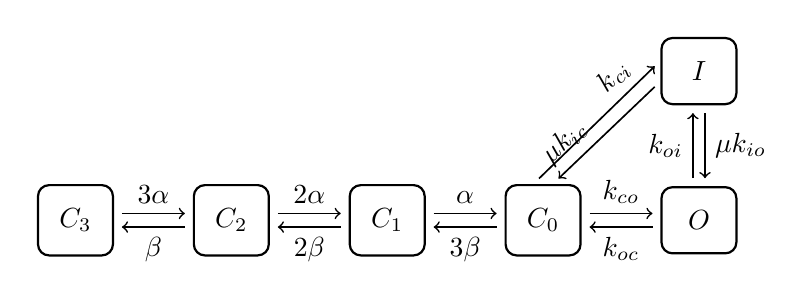
\begin{tikzpicture}[
   font=\sffamily,
   every matrix/.style={ampersand replacement=\&,column sep=1cm,row sep=1cm},
   state/.style={draw,thick,rounded corners,inner sep=.3cm},
   to/.style={->,semithick,shorten >=0.1cm,shorten <=0.1cm},
   Q/.style={->,semithick,sloped,pos=0.750000,shorten >=0.1cm,shorten <=0.1cm},  
   every node/.style={auto}]
\matrix{
\&\&\&\&\node[state] (I) {\parbox{10pt}{\centerline{$I$}}};\\
\node[state] (C_{3}) {\parbox{10pt}{\centerline{$C_{3}$}}};\&\node[state] (C_{2}) {\parbox{10pt}{\centerline{$C_{2}$}}};\&\node[state] (C_{1}) {\parbox{10pt}{\centerline{$C_{1}$}}};\&\node[state] (C_{0}) {\parbox{10pt}{\centerline{$C_{0}$}}};\&\node[state] (O) {\parbox{10pt}{\centerline{$O$}}};\\
};
\draw[to]  (O.100) to node {$k_{oi}$} (I.260);
\draw[to]  (O.190) to node {$k_{oc}$} (C_{0}.350);
\draw[to]  (I.280) to node {$\mu k_{io}$} (O.80);
\draw[Q]  (I.195) to node {$\mu k_{ic}$} (C_{0}.75);
\draw[to]  (C_{0}.10) to node {$k_{co}$} (O.170);
\draw[Q]  (C_{0}.105) to node {$k_{ci}$} (I.165);
\draw[to]  (C_{0}.190) to node {$3\beta$} (C_{1}.350);
\draw[to]  (C_{1}.10) to node {$\alpha$} (C_{0}.170);
\draw[to]  (C_{1}.190) to node {$2\beta$} (C_{2}.350);
\draw[to]  (C_{2}.10) to node {$2\alpha$} (C_{1}.170);
\draw[to]  (C_{2}.190) to node {$\beta$} (C_{3}.350);
\draw[to]  (C_{3}.10) to node {$3\alpha$} (C_{2}.170);
\end{tikzpicture}
\end{center}
\caption{Markov model of the mutant version of the sodium channel consisting of
an open state $(O)$, an inactivated state $(I)$, and four closed states
$(C_{0},C_{1},C_{2},C_{3})$. Here $\mu$ is referred to as the mutation
severity index.}%
\label{mtreac}%
\end{figure}

\bigskip


\section{Stochastic model of the sodium channel}




We use the same model of the transmembrane potential as above (see
(\ref{v1}) on page \pageref{v1}). Recall that the stochastic differential equation is
given by%
\begin{equation}
Cv^{\prime}=-g_{L}\left(  v-V_{L}\right)  -\gamma g_{Na}(v-V_{Na}), \label{sv1}%
\end{equation}
\graytable{l}{
{|c|c|} \hline
$C$ &  $1$ $\mu\text{F/cm}^{2}$\\ \hline
$g_L$ & $1/10 \text{ mS/cm}^{2}$ \\ \hline
$g_{Na}$ & $1\text{ mS/cm}^{2}$ \\ \hline
$V_L$ & $-85\text{ mV}$ \\ \hline
$V_{Na}$ & $45\text{ mV}$\\ \hline
}{Values of the parameters used in model \ref{sv1}.\label{scoef}}
where $C$ is the capacitance of the membrane, $V_{L}$ is the resting potential
of the leakage current, and $V_{Na}$ is the resting potential of the sodium
channel. The parameters are listed in Table \ref{scoef}.


%We use the following parameters:
%\begin{align}
%C  &  =1\mu\text{F/cm}^{2},\nonumber\\
%g_{L}  &  =\frac{1}{10}\text{mS/cm}^{2},\nonumber\\
%g_{Na}  &  =1\text{mS/cm}^{2}\label{scoef}\\
%V_{L}  &  =-85\text{mV,}\nonumber\\
%V_{Na}  &  =45\text{mV.}\nonumber
%\end{align}
The sodium channel can be either open (O), with $\gamma=1,$ or closed (C), with
$\gamma=0,$ and, as usual, the state of the channel is determined by a Markov
model. Since $C=1,$ we rewrite the equation in the more convenient form%

\begin{equation}
v^{\prime}=-g_{L}\left(  v-V_{L}\right)  -\gamma g_{Na}(v-V_{Na}), \label{sv2}%
\end{equation}
where $g_{L}$ and $g_{Na}$ now have the unit\footnote{The use of the odd units for 
$g_{L}$ and $g_{Na}$ stems from the fact that we have, for notational
 convenience, incorporated the capacitance of the membrane in these constants.}
$\text{ms}^{-1}.$

\subsection{A numerical scheme with an invariant region}

A numerical scheme for the model $\left(  \ref{sv2}\right)  $ can be written
in the form%
\begin{equation}
v_{n+1}=v_{n}-\Delta t\left(  g_{L}\left(  v_{n}-V_{L}\right)  +\gamma
_{n}g_{Na}(v_{n}-V_{Na}\right)  ), \label{svs}%
\end{equation}
where $\gamma_{n}$ is either zero or one and where $\Delta t$ denotes the
time step. We assume that the condition%
\begin{equation}
\Delta t<\frac{1}{g_{L}+g_{Na}} \label{svdt}%
\end{equation}
holds and, under this condition, we will show that an invariant region for the solutions
generated by the scheme $\left(  \ref{svs}\right)  $ is given by%
\begin{equation}
\Omega=\left(  V_{L},V_{+}\right)  , \label{inv_region_2}%
\end{equation}
where%
\[
V_{+}=\frac{g_{L}V_{L}+g_{Na}V_{Na}}{g_{L}+g_{Na}}
\]
and, for the parameters we defined in $\left(  \ref{scoef}\right)  $, we have
$V_{+}\approx 33.18$ mV.
%\K{zzz xxxFor parametrene definert i (\ref{scoef}) f\r{a}r jeg 
%$V_{+}\approx 28.64$mV. Men dersom $V_{Na}=45$mV som det st\r{a}r i
%bildetekseten til Figure \ref{NaM/mc.pdf} stemmer det at $V_{+}\approx 33.18$mV.}\G{Har brukt  $V_{Na}=45$mV, endret til det i dokumentet}

To derive the invariant region, we proceed along the lines used on
page \pageref{vdt} and thus start by defining%
\[
H(v,\gamma)=v-\Delta t\left(  g_{L}\left(  v-V_{L}\right)  +\gamma
g_{Na}(v-V_{Na}\right)  ).
\]
For values of $v$ in the region $\Omega$ and for values of $\Delta t$
satisfying condition $\left(  \ref{svdt}\right)$, we have the properties%
\[
\frac{d}{dv}H(v,\gamma)=1-\Delta t\left(  g_{L}+\gamma g_{Na}\right)
\geqslant1-\Delta t\left(  g_{L}+g_{Na}\right)  >0
\]
and%
\[
\frac{d}{d\gamma}H(v,\gamma)=-\Delta t\left(  g_{Na}(v-V_{Na}\right)  )>0.
\]
Using these observations, we obtain%
\[
v_{n+1}=H(v_{n},\gamma_{n})\leqslant H(V_{+},1)=V_{+}%
\]
and%
\[
v_{n+1}=H(v_{n},\gamma_{n})\geqslant H(V_{L},0)=V_{L}.
\]
So, by induction, it holds that $\Omega=\left(  V_{L},V_{+}\right)  $ is an
invariant region for scheme $\left(  \ref{svs}\right)  .$


\section[Probability density functions]{Probability density functions for the
voltage-gated channel}
The systems modeling the probability density functions in the wild type 
and mutant cases are of exactly the same form; the only difference is
given by the mutation severity index. 
The probability density functions of the states of the Markov model given in
Figure \ref{mtreac} are given by%
\begin{align}
\frac{\partial\rho_{o}}{\partial t}+\frac{\partial}{\partial v}\left(
a_{o}\rho_{o}\right)   &  =k_{co}\rho_{0}-\left(  k_{oc}+k_{oi}\right)
\rho_{o}+\mu k_{io}\rho_{i},\nonumber\\
\frac{\partial\rho_{i}}{\partial t}+\frac{\partial}{\partial v}\left(
a_{c}\rho_{i}\right)   &  =k_{oi}\rho_{o}-\mu\left(  k_{io}+k_{ic}\right)
\rho_{i}+k_{ci}\rho_{0},\nonumber\\
\frac{\partial\rho_{0}}{\partial t}+\frac{\partial}{\partial v}\left(
a_{c}\rho_{0}\right)   &  =k_{oc}\rho_{o}-\left(  k_{ci}+k_{co}+3\beta\right)
\rho_{0}+\mu k_{ic}i +\alpha \rho_{1} ,\label{vgpdf}\\
\frac{\partial\rho_{1}}{\partial t}+\frac{\partial}{\partial v}\left(
a_{c}\rho_{1}\right)   &  =2\alpha\rho_{2}-\left(  \alpha+2\beta\right)
\rho_{1}+3\beta\rho_{0},\nonumber\\
\frac{\partial\rho_{2}}{\partial t}+\frac{\partial}{\partial v}\left(
a_{c}\rho_{2}\right)   &  =3\alpha\rho_{3}-\left(  2\alpha+\beta\right)
\rho_{2}+2\beta\rho_{1},\nonumber\\
\frac{\partial\rho_{3}}{\partial t}+\frac{\partial}{\partial v}\left(
a_{c}\rho_{3}\right)   &  =-3\alpha\rho_{3}+\beta\rho_{2},\nonumber
\end{align}
where
\begin{align}
a_{o} &  =-g_{L}\left(  v-V_{L}\right)  -g_{Na}(v-V_{Na}),\label{sflux}\\
a_{c} &  =-g_{L}\left(  v-V_{L}\right)  ,\nonumber
\end{align}
with $\rho_{o}$ denoting the probability density function of being in the open
state, $\rho_{0}$ denoting the probability density function of being in the
state $C_{0},$ and so on.
%\K{zzz I de to f\o rste ligningene i dette systemet blir det brukt 
%$\rho_{c_{0}}$ i stedet for $\rho_{0}$. Er det noen grunn til det? 
%Dessuten ville jeg tro at man i tillegg til det som st\r{a}r der
%skulle legge til leddene 
%$+\alpha \rho_{1} - 3\beta \rho_{0}$ 
%p\r{a} h\o yresiden i den tredje ligningen. 
%Er det noen grunn til at man ikke gj\o r det?}
%\A{Both corrected: xxx  Glenn: make sure you correct the code accordingly.}
%\G{This was correct in the code.}

\subsection{Model parameterization}

To carry out numerical computations comparing the properties
of the  wild type and the mutant sodium channel, we need to define
the rates involved in the model described in Figure \ref{mtreac}. We use the 
rates
\[  k_{ab}(v) = k^{\infty}_{ab}(v)/\tau_{ab}, \ \ \  k_{ba}(v) = (1-k^{\infty}_{ab}(v))/\tau_{ab}, \]
with
\[k^{\infty}_{ab} = \frac{1}{1+e^{s_{a\!b}(V_{a\!b}-v)}}. \]
Furthermore, the rates $\alpha$ and $\beta$ in Figure \ref{mtreac} are given by
\[
\alpha =k^{\infty}_{cp}/\tau_{cp}  \text{ and } \beta =(1-k^{\infty}_{cp})/\tau_{cp}.
\]
With this parameterization, the principle of detailed balance is satisfied, provided that
\[ 
s_{co} + s_{ic} + s_{oi}=0 \mbox{\ \ and\ \ } s_{co}V_{co} + s_{oi}V_{oi} + s_{ic}V_{ic}  =0.  \]
The parameters are given in Table \ref{markov_rates} and we introduce the mutation as we
did in the previous chapter: We increase the probability of going from the
inactivated state to either the open or the closed state. More specifically, we define
\[
\bar{k}_{ic} = \mu k_{ic}  \text{ and } \bar{k}_{io} = \mu k_{io},
\] where, as usual, the wild type case is given by $\mu=1$. 

\begin{table}  \begin{center}
\begin{tabular}{|r|r|r|r|} \hline
$ab$ & $V_{ab}$ (mV) & $s_{ab}$ (1/mV) &  $\tau_{ab}$ (ms)\\ \hline
$co$ & -60 & 0.1& 0.01\\ \hline
$oi$ & -120 & 0.05 & 3 \\  \hline
$ic$ & -80 & -0.15& 10\\ \hline
$cp$ &-60 & 0.1& 0.1\\ \hline
\end{tabular} \end{center}
\caption{Parameters of the Markov model illustrated in Figures \ref{wtreac} 
and \ref{mtreac}. 
%\K{zzz Skal man oppgi enheter for disse parametrene?}
} 
\label{markov_rates} 
\end{table}

\subsection{Numerical experiments comparing the properties of the wild type 
and the mutant sodium channel}



In Figure \ref{NaM/pdf3.pdf}, we show the
probability density functions of the open state, the inactivated state, and the
sum of the closed states for the wild type case $(\mu=1)$ and two mutations
$(\mu=10$ and $\mu=30).$ The properties of the solutions are summarized in
Table \ref{na_stat}, which presents the expected values of the open state, the
inactivated state, and the sum of the closed states.


\fig{NaM/pdf3.pdf}{The probability density functions of the open state (left),
the sum of the closed states  (center), and the inactivated state (right) 
for the wild type case (solid line) and two values of the mutation severity 
index: $\mu=10$ and $\mu=30$. The strongest mutation differs the most
from the wild type solution. 
%{\bf xxx Glenn: something wrong here - read text and compare with headings of figures} \G{yes, fixed now.}
}

%\begin{table}  \begin{center}
%\begin{tabular}{|r|r|r|r|} \hline
%$\mu$ & $E_o$ & $E_i$ & $E_c$ \\ \hline
%1 & -50.8 & -84.9 & -83.5 \\ \hline
%10 & -13.4 & -84.9 & -57.0 \\ \hline
%30 & 13.0 & -84.9 & -20.8 \\ \hline
%\end{tabular} \end{center}
%\caption{Expected value of pdfs for WT and MT.
%{\bf xxx Glenn: Kan du legge inn $\pi_o,\pi_i,\pi_c$ i samme tabell?}}\label{na%_stat}
%\end{table}


%\begin{table}  \begin{center}
%\begin{tabular}{|r|r|r|r|r|r|r|} \hline
%$\mu$ & $\pi_o$ & $\pi_i$ & $\pi_c$ & $\rho_o$ & $\rho_i$ & $\rho_c$ \\ \hline
%1 & 0.0001 & 0.9951 & 0.0048 & -50.8 & -84.9 & -83.5 \\ \hline
%10 & 0.0002 & 0.9989 & 0.0009 & -13.4 & -84.9 & -57.0 \\ \hline
%30 & 0.0015 & 0.9941 & 0.0044 & 13.0 & -84.9 & -20.8 \\ \hline
%\end{tabular} \end{center}

\begin{table}  \begin{center}
\begin{tabular}{|r|r|r|r|r|r|r|} \hline
$\mu$ & $\pi_o\times 100 $ & $\pi_c$ & $\pi_i\times 100$ & $E_o$ & $E_c$ & $E_i$ \\ \hline
1 & 0.0067 & 0.9951 & 0.4834 & -50.8 & -84.9 & -83.5 \\ \hline
3 & 0.0080 & 0.9982 & 0.1765 & -41.1 & -84.9 & -79.6 \\ \hline
10 & 0.0162 & 0.9989 & 0.0942 & -13.4 & -84.9 & -57.0 \\ \hline
\end{tabular} \end{center}
\caption{Probability of being in the open, closed, or inactivated states and the expected value of the transmembrane
potential, provided that the channel is open, closed, or inactivated.}
%{\bf xxx Glenn xxx: Something wrong here since probability of being in inactivated state increases for increasing $\mu$.
%I guess it is ok that the channel almost certainly inactivate but that should be less likely when $\mu$ increases.
%Since numbers are small: refine mesh and refine stopping criterions?}}
\label{na_stat}
\end{table}




\subsection{Stochastic simulations illustrating the late sodium current in the mutant case}


Impaired inactivation of the sodium channel leads to a late sodium current,
which is illustrated in Figure \ref{NaM/mc.pdf}. The figure also includes 
experimental data of the sodium current taken from Bennett et al. 
\cite{Bennett1995}. We observe that, by
using $\mu=30$, the model fits the experimental data fairly well.

%\fig{NaM/mc.pdf}{Current for $\mu=1,10,30,100$.}

\begin{figure}[p]\centering
\vbox{
\includegraphics[width=0.9\linewidth]{NaM/mc.pdf}
\includegraphics[width=0.7\linewidth]{NaM/Bennet.png}
}
\caption{Currents computed using the Markov model given in Figure \ref{mtreac}. Top panel: Currents based on numerical simulations for  $\mu=1,10,30,100$. Each trace is an average of 10,000 Monte Carlo runs. The current is given by $I=g_{Na} P_o (v-V_{Na})$, with the transmembrane potential clamped at $v=0$. The currents are normalized so that the wild type case peaks at -1. The parameters are given by $V_{Na} = 45$ and $g_{Na} = 1$ and $P_o$ is the average ratio of open channels over 10,000 runs, computed at each time step. The lower graphs are from Bennett et al. \cite{Bennett1995}, for the wild type case (left) and mutant case (right). 
%\K{zzz Skal man ha med enheter her?} 
\label{NaM/mc.pdf} }
%\K{zzz Hva st\r{a}r $P_{o}$ for?}}
%\A{xxx Glenn; check that the definition $P_o$ adheres with the one you have used in code.}
%\G{$P_o$: Ratio of open channels, taken over 10000 runs.}
\end{figure}

\section[Theoretical drug for the Sodium channel]{A theoretical drug repairing the sodium channel mutation}

We introduce a theoretical drug for the sodium channel of the form given in
Figure \ref{mtreadr}. The equilibrium probabilities of the model are characterized by the equations%
\[%
\begin{array}
[c]{ccc}%
k_{ci}c_{0}=\mu k_{ic}i, & k_{oi}o=\mu k_{io}i, & k_{co}c_{0}=k_{oc}o,\\
3\beta c_{0}=\alpha c_{1}, & 2\alpha c_{2}=2\beta c_{1}, & 3\alpha c_{3}=\beta
c_{2},\\
k_{bc}b_{0}=k_{cb}c_{0}, & k_{bc}b_{1}=k_{cb}c_{1}, & k_{bc}b_{2}=k_{cb}c_{2},\\
k_{bc}b_{3}=k_{cb}c_{3}, & k_{bi}b_{i}=k_{ib}i, & k_{bo}b_{o}=k_{ob}o.
\end{array}
\]
As usual, we express all probabilities in terms of the open state probability, \label{9001}%
\begin{align*}
i &  =\frac{k_{oi}}{\mu k_{io}}o,\text{ }c_{0}=\frac{k_{oc}}{k_{co}}o,\text{
}\\
c_{1} &  =\frac{3\beta}{\alpha}\frac{k_{oc}}{k_{co}}o,\text{ }c_{2}%
=\frac{3\beta^{2}}{\alpha^{2}}\frac{k_{oc}}{k_{co}}o,\text{ }c_{3}=\frac
{\beta^{3}}{\alpha^{3}}\frac{k_{oc}}{k_{co}}o,\\
b_{0} &  =\text{ }\delta_{c}\frac{k_{oc}}{k_{co}}o,\text{ }b_{1}=\text{
}\delta_{c}\frac{3\beta}{\alpha}\frac{k_{oc}}{k_{co}}o,\text{ }b_{2}=\text{
}\delta_{c}\frac{3\beta^{2}}{\alpha^{2}}\frac{k_{oc}}{k_{co}}o,\\
b_{3} &  =\text{ }\delta_{c}\frac{\beta^{3}}{\alpha^{3}}\frac{k_{oc}}{k_{co}%
}o,\text{ }b_{i}=\delta_{i}\frac{k_{oi}}{\mu k_{io}}o,\text{ }b_{o}=\delta
_{o}o,
\end{align*}
where we have introduced the following parameters characterizing the drug:%
\[
\delta_{o}=\frac{k_{ob}}{k_{bo}},\text{ }\delta_{i}=\frac{k_{ib}}{k_{bi}%
},\text{ }\delta_{c}=\frac{k_{cb}}{k_{bc}}.
\]
Since the sum of the probabilities is one, we obtain%
\[
o_{m,d}=\frac{1}{q_{m,d}},%
\]
where the subscript indicates the mutant case in the presence of a drug. Here,%
\[
q_{m,d}=1+\frac{k_{oi}}{\mu k_{io}}+\frac{k_{oc}}{k_{co}}\left(
1+\beta/\alpha\right)  ^{3}\left(  1+\delta_{c}\right)  +\delta_{i}%
\frac{k_{oi}}{\mu k_{io}}+\delta_{o}
\]
and we recall that the wild type open probability is given by 
\[
o_{w}=\frac{1}{q_{w}},
\]
where%
\[
q_{w}=1+\frac{k_{oi}}{k_{io}}+\frac{k_{oc}}{k_{co}}\left(  1+\beta
/\alpha\right)  ^{3}.
\]
Obviously, we obtain $o_{m,d}\approx o_{w}$, provided that $q_{m,d}\approx q_{w}$.
If we choose a drug characterized by
\begin{equation}
\delta_{o}=\delta_{c}=0,\text{and }\delta_{i}=\mu-1 \label{drg_inac}%
\end{equation}
we find that%
\[
q_{m,d}=1+\frac{k_{oi}}{k_{io}}+\frac{k_{oc}}{k_{co}}\left(  1+\beta
/\alpha\right)  ^{3}=q_{w}
\]
and therefore, with the drug specified by  $\left(  \ref{drg_inac}\right)
,$ we have $o_{m,d}=o_{w}$, so the open probability at equilibrium is repaired.



\begin{figure}[ptb]
\begin{center}
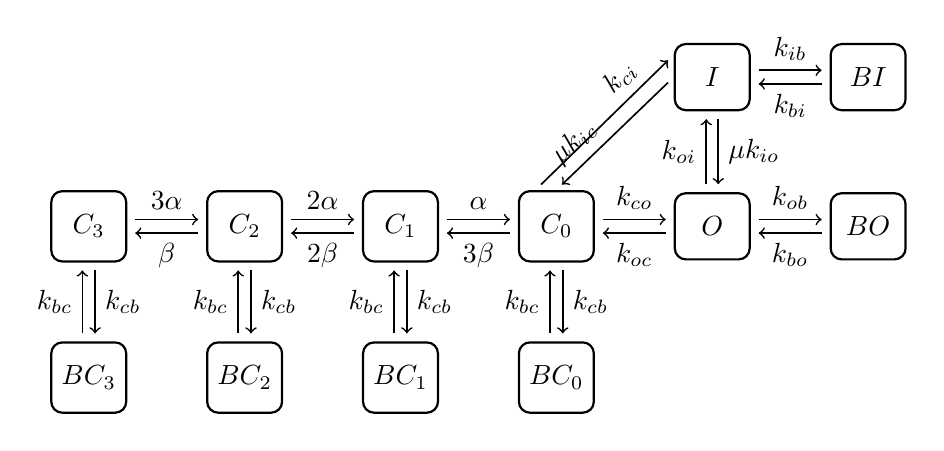
\begin{tikzpicture}[
   font=\sffamily,
   every matrix/.style={ampersand replacement=\&,column sep=1cm,row sep=1cm},
   state/.style={draw,thick,rounded corners,inner sep=.3cm},
   to/.style={->,semithick,shorten >=0.1cm,shorten <=0.1cm},
   Q/.style={->,semithick,sloped,below, above,pos=0.720000,shorten >=0.1cm,shorten <=0.1cm},  
   %Q/.style={->,semithick,pos=0.60000,shorten >=0.1cm,shorten <=0.1cm},  
   every node/.style={auto}]
\matrix{
\&\&\&\&\node[state] (I) {\parbox{10pt}{\centerline{$I$}}};\&\node[state] (BI) {\parbox{10pt}{\centerline{$BI$}}};\\
\node[state] (C_{3}) {\parbox{10pt}{\centerline{$C_{3}$}}};\&\node[state] (C_{2}) {\parbox{10pt}{\centerline{$C_{2}$}}};\&\node[state] (C_{1}) {\parbox{10pt}{\centerline{$C_{1}$}}};\&\node[state] (C_{0}) {\parbox{10pt}{\centerline{$C_{0}$}}};\&\node[state] (O) {\parbox{10pt}{\centerline{$O$}}};\&\node[state] (BO) {\parbox{10pt}{\centerline{$BO$}}};\\
\node[state] (BC_{3}) {\parbox{10pt}{\centerline{$BC_{3}$}}};\&\node[state] (BC_{2}) {\parbox{10pt}{\centerline{$BC_{2}$}}};\&\node[state] (BC_{1}) {\parbox{10pt}{\centerline{$BC_{1}$}}};\&\node[state] (BC_{0}) {\parbox{10pt}{\centerline{$BC_{0}$}}};\&\&\\
};
\draw[to]  (O.100) to node {$k_{oi}$} (I.260);
\draw[to]  (O.190) to node {$k_{oc}$} (C_{0}.350);
\draw[to]  (O.10) to node {$k_{ob}$} (BO.170);
\draw[to]  (I.280) to node {$\mu k_{io}$} (O.80);
\draw[Q]  (I.180) to node {$\mu k_{ic}$} (C_{0}.90);
\draw[Q]  (C_{0}.120) to node {$k_{ci}$} (I.150);
\draw[to]  (I.10) to node {$k_{ib}$} (BI.170);
\draw[to]  (C_{0}.10) to node {$k_{co}$} (O.170);
\draw[to]  (C_{0}.190) to node {$3\beta$} (C_{1}.350);
\draw[to]  (C_{0}.280) to node {$k_{cb}$} (BC_{0}.80);
\draw[to]  (C_{1}.10) to node {$\alpha$} (C_{0}.170);
\draw[to]  (C_{1}.190) to node {$2\beta$} (C_{2}.350);
\draw[to]  (C_{1}.280) to node {$k_{cb}$} (BC_{1}.80);
\draw[to]  (C_{2}.10) to node {$2\alpha$} (C_{1}.170);
\draw[to]  (C_{2}.190) to node {$\beta$} (C_{3}.350);
\draw[to]  (C_{2}.280) to node {$k_{cb}$} (BC_{2}.80);
\draw[to]  (C_{3}.10) to node {$3\alpha$} (C_{2}.170);
\draw[to]  (C_{3}.280) to node {$k_{cb}$} (BC_{3}.80);
\draw[to]  (BO.190) to node {$k_{bo}$} (O.350);
\draw[to]  (BI.190) to node {$k_{bi}$} (I.350);
\draw[to]  (BC_{0}.100) to node {$k_{bc}$} (C_{0}.260);
\draw[to]  (BC_{1}.100) to node {$k_{bc}$} (C_{1}.260);
\draw[to]  (BC_{2}.100) to node {$k_{bc}$} (C_{2}.260);
\draw[to]  (BC_{3}.100) to node {$k_{bc}$} (C_{3}.260);
\end{tikzpicture}
\end{center}
\caption{Markov model for a theoretical drug of the sodium channel. The model
consists of the usual states $O,I,C_{0},C_{1},C_{2}$, and $C_{3}$ and the blocked
states $BO,BI,BC_{0},BC_{1},BC_{2}$, and $BC_{3}$.}%
\label{mtreadr}%
\end{figure}




\subsection{Numerical experiments using the blocker of the inactivated state}

We have seen that a blocker of the inactivated state is a promising
candidate for repairing the mutation described in Figure \ref{mtreac}. The drug
is characterized by $\left(  \ref{drg_inac}\right)  $, so we have%
\begin{equation}
k_{ib}=\delta_{i}k_{bi}=\left(  \mu-1\right)  k_{bi} \label{kbi10}
\end{equation}
and the parameter $k_{bi}$ remains to be determined. In Table \ref{kbi_stat}, we show that the
blocker is more efficient the larger $k_{bi}$ is. In fact, the blocker is able to
repair all the relevant statistical properties of the solution. The statistical properties
presented in the table are introduced in Section \ref{statistics} on page \pageref{statistics}.


In Figure \ref{NaM/pdf_drug.pdf}, we show the open state probability density functions of the
wild type, the mutant, and the drugged version of the mutant. Again, we see
that the drug completely repairs the open state probability density function.

\fig{NaM/pdf_drug.pdf}{The open probability density function for the wild type
(WT) case and the mutant (MT) case using the mutation severity index $\mu=30$
and, finally, the mutant case with the drug given by (\ref{kbi10}) with 
$k_{bi} = 0.001\text{ ms}^{-1}$. A small value of $k_{bi}$ was used to
see a difference between the drugged case and the WT case.}

\begin{table}  \begin{center}
\begin{tabular}{|r|r|r|r|} \hline
$k_{bi}$ & $\pi_o\times 10^3 $ & $E_o$ & $\sigma_o$ \\ \hline
WT & 0.067 & -50.794 & 46.828 \\ \hline
MT & 1.534 & 12.991 & 26.831 \\ \hline
$10^{-6}$ & 1.341 & 12.940 & 26.913 \\ \hline
$10^{-5}$ & 1.180 & 12.487 & 27.634 \\ \hline
$10^{-4}$ & 0.556 & 8.240 & 33.343 \\ \hline
$10^{-3}$ & 0.135 & -16.903 & 49.326 \\ \hline
0.01 & 0.070 & -47.563 & 48.205 \\ \hline
0.1 & 0.067 & -50.729 & 46.869 \\ \hline
1 & 0.067 & -50.791 & 46.830 \\ \hline
\end{tabular} \end{center}
\caption{The open probability, $\pi_o$, the expected value of the transmembrane potential, $E_o$, and the
standard deviation, $\sigma_o$, for increasing values of $k_{bi}$. For large values of $k_{bi}$, the statistical properties 
of the mutant are completely repaired by the drug. 
}
\label{kbi_stat}
\end{table}

\subsection{The late sodium current is removed by the inactivated state blocker}


In Figure \ref{NaM/mc.pdf} above, we demonstrated, using Monte Carlo simulations, that the
mutation under consideration leads to a significant late sodium current
comparable to the current observed in experiments. By using the drug described
in $\left(  \ref{drg_inac}\right) $ with $k_{bi}=0.01 \text{ ms}^{-1},$ we see that the late
current more or less completely disappears (see Figure \ref{NaM/mc_drug}).

\fig{NaM/mc_drug}{The sodium current for the wild type (WT) and the mutant (MT)
with the mutation severity index $\mu=30$. The drug given by (\ref{kbi10}) with $k_{bi} = 0.01 \text{ ms}^{-1}$
almost completely removes the late sodium current.}


\section{Notes}

\begin{enumerate}
\item The basic structure of the Markov model in Figure \ref{wtreac} is taken 
from Patlak \cite{Patlak1991}, who discusses and evaluates several possible models in relation to experimental data.

\item Modeling the effects of a drug on the sodium channel is motivated by
the paper of Clancy et al. \cite{Clancy2007}.


\end{enumerate}



%
%
%
